% 编译：latexmk -xelatex report.tex
% 字体（均为 macOS 自带）：正文宋体，标题黑体，图表题楷体；西文正文 Times New Roman，标题 Arial，代码 Courier New
\documentclass[UTF8,a4paper,zihao=5,fontset=none]{ctexart}

\usepackage[margin=2.3cm]{geometry}
\usepackage{graphicx,booktabs,xcolor,enumitem,float,tabularx}
\usepackage[font=small,labelfont=bf,skip=6pt]{caption}
\usepackage[colorlinks,linkcolor=black,citecolor=black,urlcolor=blue!55!black]{hyperref}

\setCJKmainfont{Songti SC}[BoldFont={Songti SC Bold},ItalicFont={Kaiti SC}]   % 正文：宋体
\setCJKsansfont{Heiti SC}[BoldFont={Heiti SC Medium}]                          % 标题：黑体
\setCJKmonofont{STFangsong}                                                   % 等宽环境里的中文：仿宋
\setCJKfamilyfont{zhkai}{Kaiti SC}[BoldFont={Kaiti SC Bold}]                   % 图表题：楷体
\newcommand{\kaishu}{\CJKfamily{zhkai}}
\DeclareCaptionFont{kai}{\kaishu}
\captionsetup{font={small,kai}}
\setmainfont{Times New Roman}
\setsansfont{Arial}
\setmonofont{Courier New}[Scale=0.92]

\ctexset{
  section={format=\Large\sffamily\bfseries,beforeskip=14pt,afterskip=6pt},
  subsection={format=\large\sffamily\bfseries,beforeskip=10pt,afterskip=4pt},
  paragraph={format=\sffamily\bfseries},
}
\setlist{nosep,leftmargin=1.6em}
\setlength{\parskip}{3pt}
\graphicspath{{figures/}}   % figures with English labels
\pagestyle{plain}
\emergencystretch=2em

% 摘要：标题左对齐，正文与版心同宽
\renewenvironment{abstract}
  {\section*{摘要}}
  {\par\medskip}

\newcommand{\todo}[1]{\textcolor{red}{【待补：#1】}}
\newcommand{\code}[1]{\texttt{#1}}

\title{\sffamily\bfseries Project 1 Report\\[4pt]\Large Comparing File I/O, PostgreSQL, and openGauss}
\author{He Song \quad Student ID\ 12512808}
\date{10/07/2026}

\begin{document}
\maketitle

\begin{abstract}
本文以 IMDb 公开数据（1284 万行片名、1571 万行人名）为对象，比较了直接操作文件、使用 PostgreSQL 18.6 与使用 openGauss 6.0.0 这三种数据管理方式的速度、可靠性和资源需求等多方面的表现。与直接操作文件相比，数据库并非在所有操作上都更快：当我们把 130 万行全部改写一遍，直接重写文件只需 2.5 秒，快于其他两种数据库操作方法。数据库的优势体现在三处：一是有索引时查找一条记录只需 0.1 到 0.2 毫秒，远快于文件操作的 1.2 秒；二是更新数据时，只要能通过索引定位到目标行，时间开销就仅与被修改的行数有关，与表的总大小无关；三是进程中途被杀，数据要么全部改完、要么保持原样，不会导致意料之外的错误或者数据丢失。对项目要求的两个数据库操作方法，本文将按可靠性、资源需求和性能三项进行比较。实验结果表明，在 10 次强杀测试中，两者都没有丢失任何一笔已确认的提交，均展示出有力的可靠性；而其余两项 PostgreSQL 均占优。实验中，差距最大的是内存需求：它在 1 核 512 MB 的机器上即可带着全量数据每秒处理两万多个请求，而 openGauss 需要 2 GB 才能正常工作。此外，实验表明应用中“先读出、加一、再写回”的写法在两个数据库里会丢失同样的 86\% 的并发更新，且这一问题与选用哪个数据库无关。

\noindent\textbf{关键词：}DBMS; File I/O; PostgreSQL; openGauss; Reliability; Resource requirement
\end{abstract}

\section{引言}

当问起什么算是“更好”的时候，我第一个想法是速度。尤其是各种信息学竞赛，总要求多少多少毫秒以内，内存占用不高于多少，感觉似乎速度和内存就是全部了。但是再一细想，我已经做了好几个项目（虽然基本都是我给思路 AI 写代码），一些发在了 App Store 的单机小工具先不谈，与数据库息息相关的也有两三个了。其中一个是几周前的一场 500 人的黑客松比赛，我负责选手小程序的开发，一个很重要的功能就是进行身份的核对签到，确认对方是有资格参加比赛的参赛选手。还有一个是接的单子，开发一个校园论坛的微信小程序，需要登录注册，更需要同时展示大量的图片文字等信息流。

而手里正在做的，是我正在给树仁书院做的学习搭子匹配系统\footnote{\url{https://github.com/QianMo0729/shuren-study-buddy}}。它要成批录入账号，用校园邮箱验证码激活，再按问卷给每两个人计算匹配分。

这些项目决定了我怎样理解作业提出的两个问题：

\begin{description}[leftmargin=3.4em,labelwidth=2.8em,labelsep=0.6em]
  \item[RQ1] 与直接操作文件相比，DBMS 提供了什么？
  \item[RQ2] PostgreSQL 和 openGauss 哪个更好，按什么标准？
\end{description}

所以对于数据的管理，我不能只看谁跑得快。我认为对我手头这些小型服务，“好”按重要程度排下来是：

\begin{enumerate}
  \item \textbf{可靠性。}数据不能错、不能丢。还要能在高并发下保证多人同时写不出错；哪怕服务器突然宕机，也要保证不出错不丢数据。
  \item \textbf{资源需求。}小机器要跑得动。我的服务器只有 2 核 2 GB，必须要足够精简，内存和 CPU 的要求都不能太高。
  \item \textbf{性能。}需要在保证速度的情况下能尽可能的满足高并发高吞吐的实际使用需求。
\end{enumerate}

为了回答这两个问题，我写了一套测试程序，在文件、PostgreSQL 和 openGauss 上执行同样的操作，先核对三者的结果一致，再比较运行时间和运行开销。实验在一台 16 英寸 MacBook Pro 上进行，搭载 Apple M5 Pro 芯片和 24 GB 统一内存。为测试不同资源条件下的表现，我将同一台虚拟机设置为五种不同规格，配置范围从 1 核 CPU、512 MB 内存 到 4 核 CPU、8 GB 内存。

本文其余部分安排如下：第 \ref{sec:background} 节介绍解释实验结果所需的机制；第 \ref{sec:design} 节说明数据、环境和实验内容；第 \ref{sec:file}、\ref{sec:pgog} 节分别给出 RQ1 和 RQ2 的结果；第 \ref{sec:discussion} 节讨论这些结果对我自己的选择意味着什么；第 \ref{sec:threats} 节列出局限；第 \ref{sec:conclusion} 节总结。

\section{背景}\label{sec:background}

\paragraph{文件}文件操作实际上只是交给程序一串字节。如果要找一条记录，程序需要一直读到出现为止。由于后面的内容都要跟着挪动，所以一个值的改变没法直接改。更新是否会造成崩溃、多个写入者会不会互相干扰，需要由程序本身来决定。在本实验中，我将使用 Java I/O 来进行直接的文件操作。

\paragraph{PostgreSQL}PostgreSQL 把行存在堆表里，采用多版本并发控制：更新会写入该行的一个新版本，旧版本留待 \code{VACUUM} 回收 \cite{pgmvcc}。修改在写入数据文件之前先记入预写日志，崩溃后靠它恢复 \cite{pgwal}。默认的索引是 B-tree；\code{pg\_trgm} 扩展提供三元组索引，可以服务以通配符开头的 \code{LIKE} 匹配 \cite{pgtrgm}。顺序扫描可以分给多个并行进程，默认每个查询 2 个 \cite{pgparallel}。

\paragraph{openGauss}openGauss 是华为开源的关系数据库 \cite{ogdocs,ogsrc}，内核源自 PostgreSQL：在我的测试中，它上报的 \code{server\_version} 仍是 9.2.4。它的 SQL 方言与 PostgreSQL 大体兼容，但有自己的驱动和工具，也有几处与本文相关的差异。除了继承自 PostgreSQL 的追加写堆表，它还提供原地更新的存储引擎 Ustore。并行执行默认关闭，要调大 \code{query\_dop} 才启用。新建的数据库默认是 Oracle 兼容模式，需要显式指定才是 PostgreSQL 兼容模式。

\section{实验设计}\label{sec:design}

\subsection{数据集}

我使用的是 IMDb 公开的三张表 \cite{imdb}，包含片名和人名（表 \ref{tab:data}）。规模 s 和 规模 m 是从全量数据集中随机抽取的。

\begin{table}[H]
\centering\small
\caption{实验数据。清洗后的文件采用 PostgreSQL COPY 的文本格式，Java 文件程序和两个数据库读的是同一份字节。}
\label{tab:data}
\begin{tabular}{lrrrl}
\toprule
规模 & 片名表 & 人名表 & 评分表 & 来源 \\
\midrule
s & 127,865 & 156,787 & 17,065 & 1\% 抽样 \\
m & 1,285,110 & 1,573,840 & 171,407 & 10\% 抽样 \\
l & 12,842,753 & 15,712,491 & 1,718,051 & 全量（片名文件 1.0 GB，人名文件 0.9 GB） \\
\bottomrule
\end{tabular}
\end{table}

\subsection{实验环境与虚拟机规格}

所有实验跑在我自己的电脑——一台 16 英寸 MacBook Pro，搭载 Apple M5 Pro 芯片和 24 GB 统一内存，型号 A3428——上的一台 Linux 虚拟机里，使用系统Ubuntu 24.04，arm64 版本。PostgreSQL 版本 18.6，openGauss 版本 6.0.0，均使用 Docker 镜像。

我把整台虚拟机缩到指定大小模拟。虚拟机每次重启成指定的 CPU 数和内存，总共分为五档：1 核 512 MB、1 核 1 GB、2 核 2 GB、2 核 4 GB、4 核 8 GB，以模仿有限预算下不同轻量服务器的规格。

\subsection{实验内容}

表 \ref{tab:workloads} 列出了全部实验。检索、批量更新、更新中途崩溃和并发计数这四项在文件和两个数据库上都进行了实验模拟，其余实验只在数据库上进行。

\begin{table}[H]
\centering\small
\caption{实验一览。“4/8”“2/2”是测数据库时虚拟机的规格（CPU 核数/内存 GB）。文件程序一律在 4/8 上运行。}
\label{tab:workloads}
\begin{tabularx}{\linewidth}{@{}l>{\raggedright\arraybackslash}Xll@{}}
\toprule
实验名 & 实验内容 & 虚拟机 & 次数 \\
\midrule
检索 & 按 id、精确值、前缀、子串查找片名，分无索引和有索引 & 4/8 & 预热 2 次 + 计时 5 次 \\
批量更新 & 把人名里的 T 换成 Ttt：所有含 T 的行，或指定的 10 行 & 4/8 & 3 到 5 次 \\
更新中途崩溃 & 批量更新做到一半时杀掉写入进程，检查数据 & 2/2 & 每个系统 3 次 \\
并发计数 & 8 个客户端同时给同一个计数器加 1 & 2/2 & 3 次 \\
重复插入 & 16 个客户端同时插入同一个主键，共 300 轮 & 2/2 & 1 次 \\
负载下崩溃 & 8 个客户端持续提交 3 行的事务，8 秒后 \code{kill -9}，逐笔核对已确认的提交 & 2/2 & 每个系统 5 次 \\
并发压测 & 1、4、16、64 个并发各 20 秒；只读，或八成读两成写 & 4/8 & 3 轮 \\
持续负载 & 16 个并发，八成读两成写，连续 10 分钟 & 2/2 & 1 次 \\
规格阶梯 & 16 个并发，八成读两成写，五种规格各 30 秒 & 全部 & 每格 1 次 \\
\bottomrule
\end{tabularx}
\end{table}

\subsection{公平性措施}

\begin{itemize}
  \item \textbf{先进行结果核对。}每个查询都记录返回行数和 id 校验和，每次更新都记录改动行数、总行数、人名总字节数。文件、PostgreSQL、openGauss 三方共 72 项核对，确保全部一致后再进行时间的比较。
  \item \textbf{三者在同一台虚拟机、同一块盘上。}Java 文件程序和 JDBC 客户端都放进虚拟机里跑。在两个数据库进行比较时，压测客户端放在虚拟机外面，防止它占用被测机器的 CPU 造成结果不准确。
  \item \textbf{两个数据库的条件对齐。}均使用 UTF-8 和 C 排序规则，字符串比较为逐字节比较，与 Java 的 \code{equals} 一致。内存参数按机器大小设置一致（\code{shared\_buffers} 取内存的四分之一），\code{fsync} 和同步提交始终开启。
  \item \textbf{重复测量。}查询先预热 2 次再计时 5 次，取中位数；并发压测两个库轮流跑 3 轮。
\end{itemize}

\subsection{程序实现}

文件操作使用四个 Java 程序：\code{FileSearch} 用 \code{BufferedReader} 逐行扫描；\code{MemIndex} 把 id 和片名读进数组、排好序，再二分查找；\code{FileUpdate} 重写文件，正确的做法是写临时文件、\code{fsync}、再进行原子改名，另外留了一个“读进内存后原地覆盖”的写法专门用来演示意外情况；\code{FileCounter} 做并发计数。数据库则通过 JDBC 执行同样的操作（\code{DbSearch}、\code{DbUpdate}），外加压测程序 \code{DbLoadTest} 和可靠性测试 \code{DbReliability}。同一份 Java 代码跑两个库，仅有连接串和驱动、批量导入用的 COPY 接口、建库语句这三处不同。

\section{结果：DBMS 与文件操作的对比}\label{sec:file}

\subsection{检索}

\begin{figure}[H]
\centering
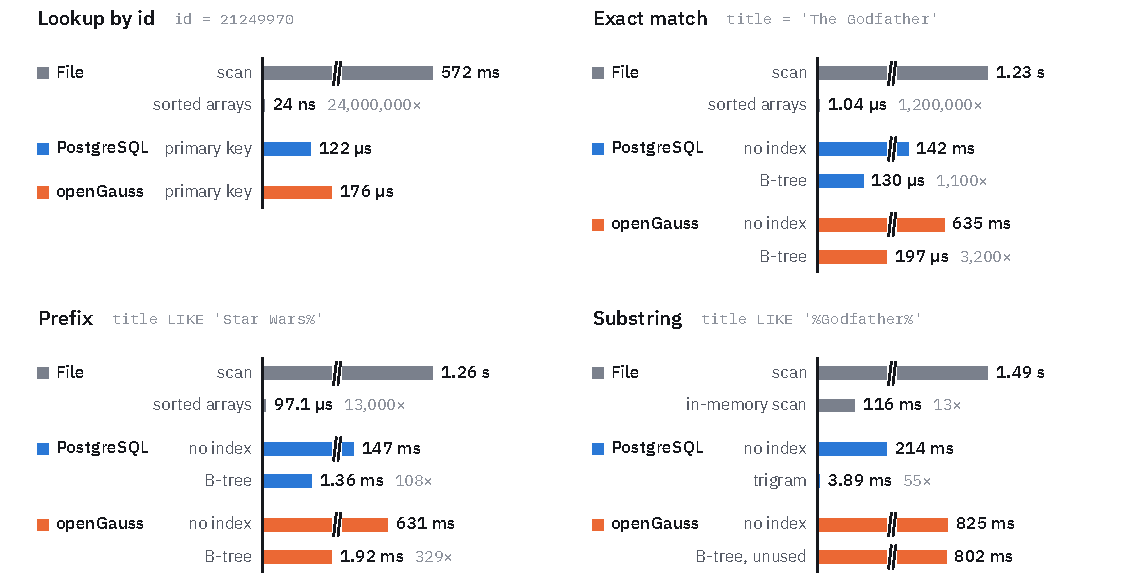
\includegraphics[width=\linewidth]{fig01_retrieval.pdf}
\caption{在 1284 万行片名上做四种查找的耗时（5 次的中位数）。灰色小字表示相对上一行快的倍数。}
\label{fig:retrieval}
\end{figure}

没有索引时，三者都需要把 1284 万行读一遍（图 \ref{fig:retrieval}）。当使用文件直接操作时，扫一遍需要 1.2 到 1.5 秒；openGauss 需要 0.6 到 0.8 秒，手动打开并行（\code{query\_dop=3}）后降低至 0.23 秒；PostgreSQL 默认并行需要 0.14 到 0.21 秒，关掉并行后需要 0.40 秒；

建了 B-tree 索引后，精确匹配降到 0.13 毫秒（PostgreSQL）和 0.20 毫秒（openGauss），快了一千到三千倍。并且在三种数据规模下时间几乎一致。

为了对文件操作进行加速，我把 id 和片名读进内存、排好序，最后二分查找一次只要 1 微秒，比数据库还快两个数量级，因为省掉了网络往返和 SQL 解析。这也印证了前文所叙的通过程序进行文件操作与程序本身的写法相关。

而对于子串匹配（\verb|LIKE '%Godfather%'|），由于 PostgreSQL 有三元组索引，214 毫秒降到 3.9 毫秒；但因为 openGauss 6.0.0 没带这个扩展，只能进行全表扫描，速度较慢。

\subsection{批量更新}

\begin{figure}[H]
\centering
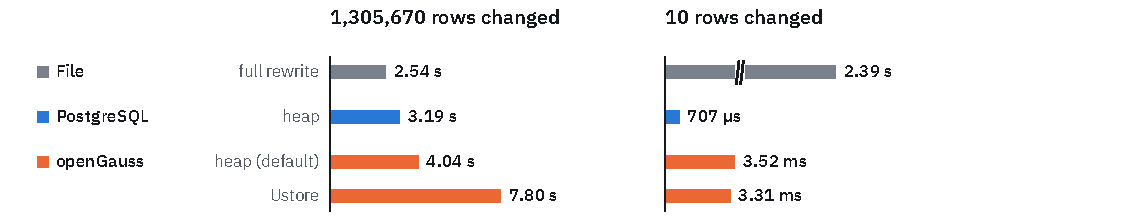
\includegraphics[width=\linewidth]{fig03_bulk_update.pdf}
\caption{把 1571 万个人名里的 T 换成 Ttt 的耗时，含提交和落盘。左：所有含 T 的行；右：只改指定的 10 行。}
\label{fig:update}
\end{figure}

在文本文件里，一个值变长了没法原地改，所以不管改多少行都要整份重写，因此需要 2.4 到 2.5 秒（图 \ref{fig:update}）。而数据库只动涉及的行：在改 10 行的情况下，PostgreSQL 只需要 0.7 毫秒，openGauss 3.5 毫秒。

在极限边界情况下会出现一些反常。改 130 万行时文件操作最快，仅需要 2,54 秒。而 PostgreSQL 使用了 3.2 秒，openGauss 花费了 4.0 秒。原因是文件只需要从头到尾写一份新的；数据库除了写新行，还要保留旧版本、写预写日志。因此当需要操作的数据占据的比例较大时，可能直接使用文件操作会更加便捷。（也许下一个 Project 就是探究这个比例？）

换成 openGauss 的原地更新引擎 Ustore 后，同样的更新之后表只涨了 24 MB，两个库的普通堆表都涨了约 100 MB，而且 \code{VACUUM} 之后文件也不会缩回去。但是这次更新它用了 7.8 秒，两倍于堆表所需要的时间。

\subsection{崩溃时的数据完整性}

\begin{figure}[H]
\centering
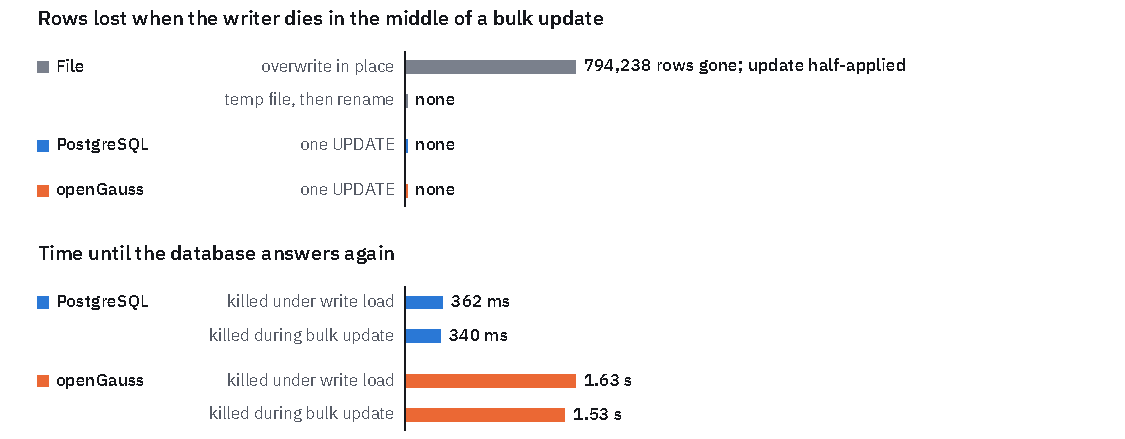
\includegraphics[width=\linewidth]{fig10_crash.pdf}
\caption{上：批量更新进行到一半时进程被 \code{kill -9}，事后数据的状态（157 万行的人名表）。下：数据库被杀后重启，到能重新回答查询的时间（中位数）。数据库部分在 2 核 2 GB 上测得。}
\label{fig:crash}
\end{figure}

最省事的改文件写法是“读进内存，改完，写回原文件”。我让它写到一半时把进程杀掉：157 万行只剩 78 万行，剩下的里面有 6 万多行已经改过。这份文件既不是旧的也不是新的，没法知道哪些改了。

先写临时文件、落盘、再改名的写法没有这个问题，原文件完好。同样的测试对数据库各做 3 次，\code{UPDATE} 执行到一半时杀掉服务进程，重启后表和更新前一模一样（图 \ref{fig:crash} 上）。

而数据库则是在使用默认语法完成写入时直接杀进程也没有任何问题，文件数据没有丢失，作为商业上广泛使用的语言，这很好的避免了写代码时“学艺不精”或者单纯因粗心没有写好写入操作导致的数据丢失问题。

顺手，我也统计了数据库被杀后重启，到能重新回答查询的时间（中位数）。

\subsection{并发写入的正确性}

\begin{figure}[H]
\centering
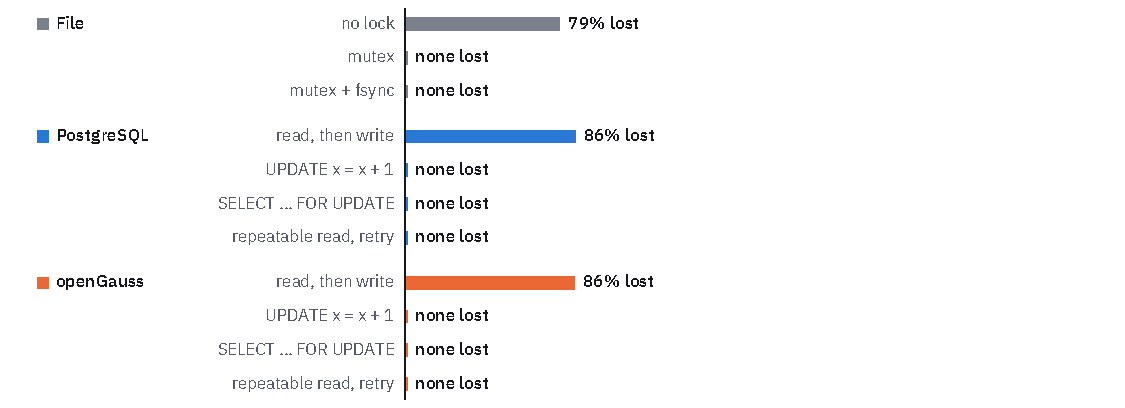
\includegraphics[width=\linewidth]{fig09_lost_updates.pdf}
\caption{8 个客户端同时给同一个计数器加 1，最后少了多少。文件共 16,000 次加一，数据库共 8,000 次，各 3 轮取中位数。}
\label{fig:lost}
\end{figure}

8 个线程同时对文件里的一个计数器进行“读、加一、写回”的操作，不加锁时 79\% 的“加一”丢了（图 \ref{fig:lost}）。我们可以通过加入互斥锁来改善这个情况，但互斥锁只在一个进程内有效，换成两个进程又得重新想办法，不利于维护和拓展。

而在数据库里用一条 \code{UPDATE x = x + 1}，一次都不丢。但如果应用代码照着文件的思路写，先 \code{SELECT} 出来、加一、再 \code{UPDATE} 回去，两个数据库丢掉同样的 86\%。

想到黑客松的签到查重，我又添加了一个并发同账号写入的模拟测试环境。我让 16 个客户端同时插入同一个主键，重复 300 轮：两个数据库每轮都恰好接受 1 个、拒绝 15 个，没有重复写入的问题，可以使用数据库及其简单的语法就能完成，而文件操作需要开发者进行严格的约束，此处不再赘述。

\section{结果：PostgreSQL 与 openGauss 的对比}\label{sec:pgog}

\subsection{可靠性}

在 2 核 2 GB 上，我让 8 个客户端不停提交事务（每笔写 3 行），8 秒后用 \code{kill -9} 杀掉数据库，每个库 5 次。客户端只在 \code{COMMIT} 成功返回后才把事务号记下来。重启后逐笔核对：PostgreSQL 的 611,802 笔、openGauss 的 233,803 笔已确认提交全部都在，也没有任何一笔只写了一半。

差别在重启后的恢复时间：PostgreSQL 约 0.36 秒，openGauss 约 1.6 秒（图 \ref{fig:crash} 下）。

\begin{figure}[!htb]
\centering
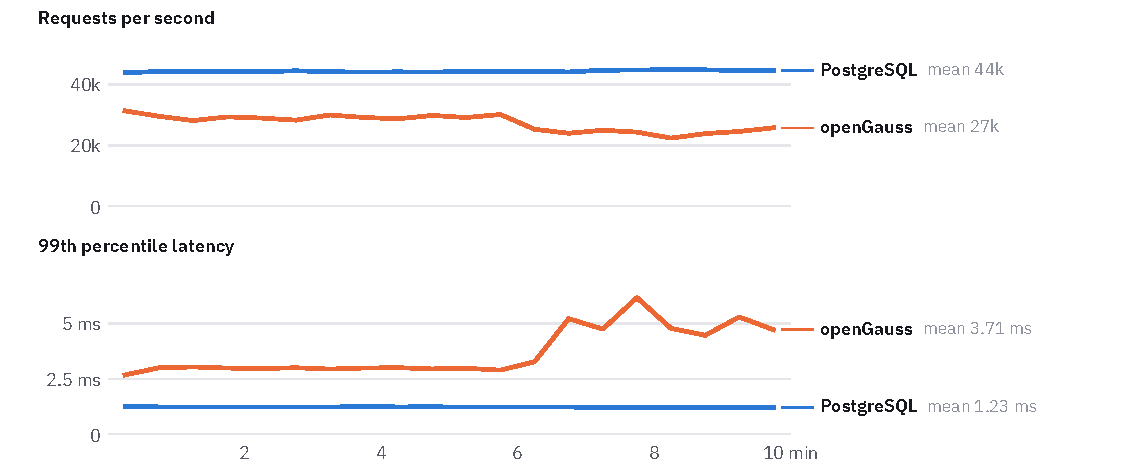
\includegraphics[width=\linewidth]{fig08_sustained_load.pdf}
\caption{2 核 2 GB、全量数据、16 个并发（八成读、两成写）连续跑 10 分钟，每 30 秒一个点。}
\label{fig:soak}
\end{figure}

另一个差别要跑久一点才看得到（图 \ref{fig:soak}）。同样的负载连续跑 10 分钟，两者都没有一个失败请求。PostgreSQL 一直稳定在每秒 4.4 万次。openGauss 平均每秒 2.7 万次，第 6 分钟之后明显变慢，最后两分钟比最初两分钟低 18\%，p99 延迟从 3 毫秒升到 5 毫秒左右，最慢的一个请求等了 1.6 秒（PostgreSQL 是 30 毫秒）。我没有查清原因，猜测和检查点或脏页回写有关，这里只报告现象。

我原来还想比“出错时的提示清不清楚”。试了重复主键、类型不符、语法错误等 10 种情况，两个库返回的 SQLSTATE 完全相同，文字也几乎一样，这一项分不出高下。

\subsection{资源需求}

\begin{figure}[H]
\centering
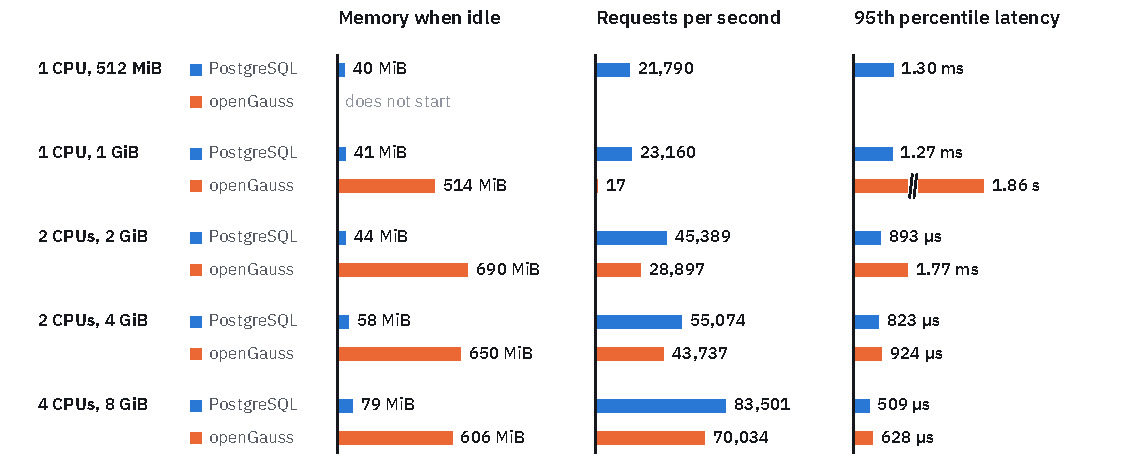
\includegraphics[width=\linewidth]{fig06_server_requirements.pdf}
\caption{把虚拟机缩到不同大小后的表现：全量数据，16 个并发，八成读、两成写，内存参数已按机器大小调好。每格测一次（30 秒负载）。}
\label{fig:ladder}
\end{figure}

图 \ref{fig:ladder} 是我最关心的结果。

PostgreSQL 在最小的 1 核 512 MB 上就能带着全量数据每秒处理 2.2 万个请求，空闲时只占 40 MB。

openGauss 在 512 MB 上起不来。即时把内存参数调小了，进程启动时也会直接崩溃（退出码 139），内核日志里是一句“not enough memory for the allocation”。1 GB 上它能启动，但空闲占用为 514 MB，一加负载每秒只有 17 个请求。这种情况到 2 GB 才正常：每秒 2.9 万次，同一台机器上 PostgreSQL 是 4.5 万次。因此在价格上，要买一台能正常运行 PostgreSQL 的最低配服务器大概能够比一台能正常运行 openGauss 的最低配服务器便宜一半。

还有一个容易踩的地方。openGauss 安装时会按当时机器的大小选内存参数，在 8 GB 机器上装好的实例默认要申请 3.3 GB 共享内存。我把这样一个实例原样搬到 2 GB 的机器上，它直接启动失败，必须先改参数。PostgreSQL 无论在哪装，默认的共享缓冲区都是 128 MB，搬到哪都一样，这样也降低了服务器的迁移成本。

\subsection{性能}

\begin{figure}[H]
\centering
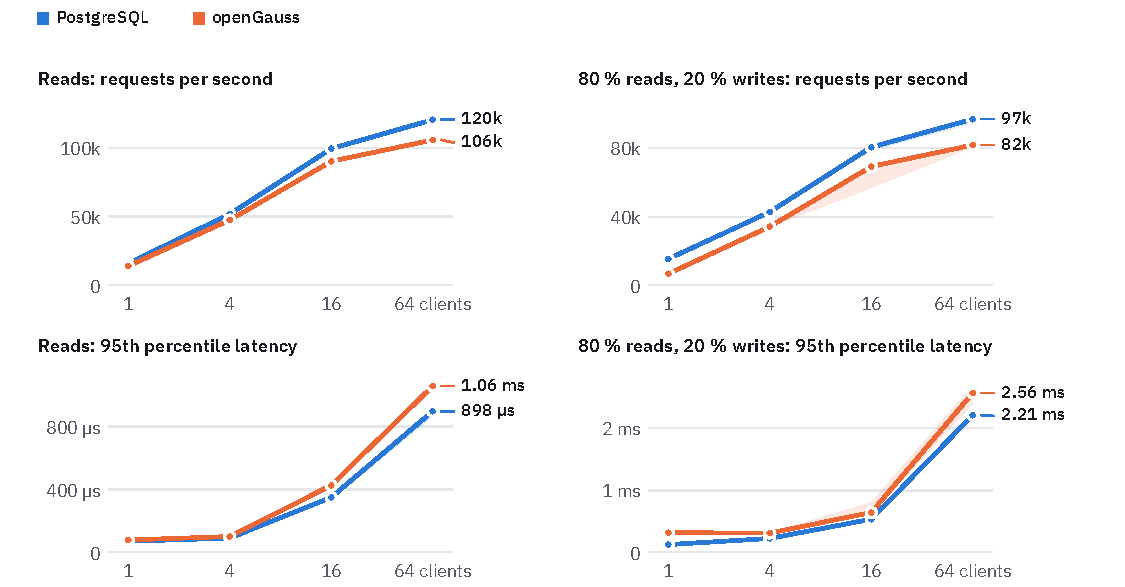
\includegraphics[width=\linewidth]{fig05_concurrent_load.pdf}
\caption{4 核 8 GB、全量数据下的吞吐和 p95 延迟。线是 3 轮的中位数，浅色带是最低到最高。读是按主键取一条片名，写是给一条评分的票数加一。}
\label{fig:load}
\end{figure}

当并发测试从 1 加到 64时，两者的曲线形状很像（图 \ref{fig:load}）。64 并发时 PostgreSQL 每秒 12.0 万次只读、9.7 万次读写混合，比 openGauss 分别高 14\% 和 18\%，全程没有失败请求。单个客户端做读写混合时差得更多，每秒 1.55 万对 0.69 万。

导入数据时差距也不小：1284 万行片名，PostgreSQL 用 \code{COPY} 导入花 5.3 秒，openGauss 25.3 秒；建同一个 B-tree 索引是 2.6 秒对 12.2 秒，索引大小是 314 MB 对 498 MB。

\subsection{兼容性与迁移成本}

同一套 SQL 在两边基本都能跑，但是 openGauss 新建的数据库默认是 Oracle 兼容模式，空字符串会被当成 \code{NULL}，需要显式写 \code{DBCOMPATIBILITY 'PG'} \cite{ogdocs}。它得用自己的 JDBC 驱动。它没有 \code{pg\_trgm}，所以子串检索没有索引可用。再加上 7.0 镜像起不来，这些兼容性的问题都需要努力的 Debug，虽然现在有 AI 的参与（是不是该叫 SI 了），但是差一点的 AI 比如你豆包豆姐我猜大概秃头了都发现不了问题（。

\section{讨论}\label{sec:discussion}

\paragraph{RQ1：DBMS 相对文件提供了什么。}不是单纯的速度。把文件读进内存排好序，查找比两个数据库都快；整份重写文件，在大批量更新上也比两者快。DBMS 提供的是：快而且安全的做法不必由应用自己编写和维护。索引存在磁盘上并保持最新，小改动只花小代价，中断的修改不留痕迹，不管多少客户端同时写，唯一性都有保证。这些在文件上都能实现，临时文件加改名的写法就是例子，但每实现一样，程序里就多一处可能出错的地方。作为广泛的需要在商业上使用的东西，它能够自动地规避一些常见的错误和坑，防止业余程序员（和弱智的AI？）乱写的代码把系统弄崩溃、把数据弄丢。

\paragraph{RQ2：PostgreSQL 还是 openGauss。}按我的三条标准，PostgreSQL 更好。可靠性上两者都没丢数据，但是 PostgreSQL 恢复更快，长时间负载下更稳。资源需求上差距最大：在 2 核 2 GB 的机器上，PostgreSQL 空闲时占的内存不到 openGauss 的十分之一，而且在内存只有四分之一的机器上照样能用。性能上它领先一到两成。所以学习搭子系统我会用 PostgreSQL。我自己那台 2 核 2 GB 的服务器两者都能跑，但 openGauss 空闲就要 690 MB，如果应用也部署在同一台机器上，剩下的就不多了。

尽管如此，这不等于 openGauss 不好。它的 Ustore 在频繁更新的表上明显省空间，并行查询打开后全表扫描也快了近三倍。如果机器有 4 GB 以上、又有人专门调参数，两者的差距会小很多，甚至在某些表现上更强。（华为就是不差钱哈）

\section{局限性}\label{sec:threats}

\begin{itemize}
  \item 测试在笔记本的虚拟机里完成，CPU 和固态硬盘都比普通云服务器快得多，并且使用的是 Arm 架构的 Apple 芯片，在 X86 的指令集下结果是否会有反转无法确定。
  \item 虚拟机里的 \code{fsync} 不保证数据真的到了物理磁盘，所以崩溃测试覆盖的是进程被杀，但不能保证在直接断电的情况下是否会造成数据的丢失、磁盘的损伤等。
  \item 图 \ref{fig:ladder} 每一格只测了一次。方向很清楚，具体数字的波动没有量化。
  \item 压测用的请求很简单，只有按主键读和单行更新。复杂查询多的业务，结论可能不同。
  \item 每个系统只测了一个版本。由于测试期间我的电脑可能有后台活动，不能保持完全相同的情况。不过并发压测 3 轮之间的差距基本在 2\% 以内。
\end{itemize}

\section{结论}\label{sec:conclusion}

我在同样的 1284 万行片名和 1571 万行人名上比较了文件、PostgreSQL 18.6 和 openGauss 6.0.0，并核对了三者的结果完全一致。和文件相比，DBMS 并没有赢下每一项测量，但它让带索引的查找、小范围更新、崩溃安全和并发下的唯一性成了默认行为，不用程序自己去保证。两个数据库在 10 次强杀中都保住了每一笔已确认的提交；PostgreSQL 恢复更快，只需四分之一的内存就能运行，速度快一到两成，所以在我目前接触到的业务场景中，我会倾向于选择 PostgreSQL 为“更好”的选择。

\begin{thebibliography}{9}\small
\bibitem{pgmvcc} PostgreSQL Global Development Group. \emph{PostgreSQL 18 Documentation: Concurrency Control}. \url{https://www.postgresql.org/docs/18/mvcc.html}（2026 年 10 月访问）.
\bibitem{pgwal} PostgreSQL Global Development Group. \emph{PostgreSQL 18 Documentation: Write-Ahead Logging}. \url{https://www.postgresql.org/docs/18/wal-intro.html}（2026 年 10 月访问）.
\bibitem{pgtrgm} PostgreSQL Global Development Group. \emph{PostgreSQL 18 Documentation: pg\_trgm}. \url{https://www.postgresql.org/docs/18/pgtrgm.html}（2026 年 10 月访问）.
\bibitem{pgparallel} PostgreSQL Global Development Group. \emph{PostgreSQL 18 Documentation: Parallel Query}. \url{https://www.postgresql.org/docs/18/parallel-query.html}（2026 年 10 月访问）.
\bibitem{ogdocs} openGauss Community. \emph{openGauss Documentation}. \url{https://docs.opengauss.org/en/}（2026 年 10 月访问）.
\bibitem{ogsrc} openGauss Community. \emph{openGauss-server source repository}. \url{https://gitee.com/opengauss/openGauss-server}（2026 年 10 月访问）.
\bibitem{imdb} IMDb. \emph{IMDb Non-Commercial Datasets}. \url{https://developer.imdb.com/non-commercial-datasets/}（2026 年 10 月访问）.
\end{thebibliography}

\appendix
\section{复现方法}

代码和全部实验结果公开在\ {\def\UrlBreaks{\do\/\do\-}\url{https://github.com/QianMo0729/Principles-of-Database-Systems-H-/tree/main/Project1}}。代码分三部分：\path{Codes/java} 是测量程序，\path{Codes/scripts} 是每个实验一个脚本，\path{Codes/analysis} 负责汇总和作图。装好 Colima 和 Docker 后执行 \path{Codes/scripts/run_all.sh} 即可从下载数据跑到出图，约两小时。全部原始测量值在 \code{output/vm-<规格>/raw/} 下，汇总表在 \path{output/summary/RESULTS.md}。由于 IMDb 数据只允许个人和非商业使用且公开可下载，所以我只放了下载脚本。

\end{document}
